
%=========================================================
\section{Módulos del sistema}

La aplicación se encuentra organizada en módulos, con la finalidad de agrupar y administrar de mejor manera los requerimientos funcionales del sistema. Dividir el sistema en módulos permite visualizar e identificar rápidamente aquellos aspectos funcionales que pueden tratarse conjuntamente. La figura \ref{fig:modulos} muestra los módulos propuestos para la aplicación.

\begin{figure}[h!]
	\begin{center}
		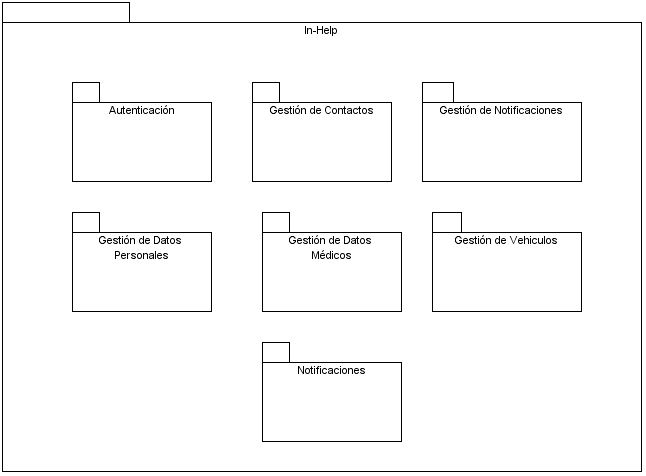
\includegraphics[scale=0.4]{ModeloComportamiento/imagenes/modulosSistema.png}
		\caption{Módulos del sistema.}
		\label{fig:modulos}
	\end{center}
\end{figure}

A continuación se describen de manera general cada uno de los módulos:

\begin{itemize}
	\item {\bf Autenticación:} Agrupa los casos de uso que tienen que ver con el proceso de registro de usuario para la aplicación, así como para el inicio de sesión una vez que el usuario se encuentra registrado.
	
	\item {\bf Gestión de Contactos:} Agrupa los casos de uso que tienen que ver con el proceso de registro y gestión de contactos para un usuario, el usuario puede agregar, consultar, editar y eliminar la información de los contactos registrados en la App.
	
	\item {\bf Gestión de Notificaciones:} Agrupa los casos de uso que tienen que ver con el proceso de configuración y gestión de notificaciones para un usuario, el usuario puede consultar, editar y eliminar la información de notificaciones si es que así lo desea.
	
	\item {\bf Gestión de Datos Personales:} Agrupa los casos de uso que tienen que ver con el proceso de registro y gestión de datos personales para un usuario, el usuario puede agregar, consultar, editar y eliminar su información personal que se encuentre registrada en la App.
	
	\item {\bf Gestión de Datos Médicos:} Agrupa los casos de uso que tienen que ver con el proceso de registro y gestión de datos médicos para un usuario, el usuario puede agregar, consultar, editar y eliminar la información médica personal que se encuentre registrada en la App.
	
	\item {\bf Gestión de Vehículos:} Agrupa los casos de uso que tienen que ver con el proceso de registro y gestión de vehículos para un usuario, el usuario puede agregar, consultar, editar y eliminar la información de los vehículos registrados en la App.
\end{itemize}